\externaldocument{../appendix/chapter_app}
\startchapter{Modeling}
\label{chapter:Mod}
I investigated some common used communication methods divide the communication methods into two categories based on their data transmission properties. Based on this investigation, I modelled the communication of two programs. I also the dual-trace of two communicating programs in the perspective of communication analysis. These two models are the foundation to decide how communications being identified from the dual-trace and how to present them to the user.

\section{Communication Categorization and Communication Methods}
The goal of this work is to identify the communications from the dual-trace. We need to understand the properties of the communications to identify them. In general, there are two types of communication: reliable and unreliable in the perspective of their reliability of data transmission. The reason to divide the communication methods into these two categories is that the data transmission properties affect the mechanism of the identification of the communications fall in different categories. In the following two subsections, I summarize the characteristics of these two communication categories. The communication methods list in Table\ref{methodsInCategories} will be discussed further to provide more concrete comprehension. 
\begin{table}[H]
\centering
\caption{Communication Methods Discussed in This Work}
\label{methodsInCategories}
\begin{tabular}{|l|l|}
 \hline
\textbf{Reliable Communication}& \textbf{Unreliable Communication}\\
 \hline
Named Pipes & Message Queue   \\
TCP &  UDP \\
 \hline
\end{tabular}
\end{table}


\subsection{Reliable Communication}\label{reliable}
A reliable communication guarantees the data being sent by one endpoint of the channel always received losslessly and in order to the other endpoint. With this property, the send data union in the send stream of one endpoint should equal to the receive data union in the receive stream of the other endpoint. The send data union is the conjunction of the data trunks in all send events in the send stream by the event time ordering. The receive data union is the conjunction of the data trunks in all receive events in the receive stream by the event time ordering. Therefore, the send and receive data verification should be in send and receive stream level by comparing the send data union of one endpoint to the receive data union of another. For some communication methods, a channel can be closed without waiting the completion of all data transmission. In this case, the receive data union can be a sub string of the send data union.

\subsection{Unreliable Communication}\label{unreliable}
An unreliable communication does not guarantee the data being send always arrive the receiver. Moreover, the data packets can arrive to the receiver in any order. However, the bright side of unreliable communication is that the packets being sent are always arrived as the origin packet, no data re-segmentation would happen. Accordingly, the send and receive data verification should be done by matching the data packets in a send event to a receive event on the other side.

\subsection{Communication Methods}
In this section, I describe the mechanism and the basic data transfer characteristics of each communication method in Table\ref{methodsInCategories} briefly. Moreover, data transfer scenarios are represented correspondingly in diagrams for each communication method. 
 
\subsubsection{Named Pipe}
In computing, a named pipe provides FIFO communication mechanism for inter-process communication. It allows two programs send and receive message through the named pipe.

The basic data transfer characteristics of Named Pipe are:
\begin{itemize}
  \item Bytes received in order
  \item Bytes sent as a whole trunk can be received in segments
  \item No data duplication
  \item Only the last trunk can be lost
\end{itemize}

Based on these characteristics, the data transfer scenarios of Named pipe can be summarized in Figure\ref{namedpipe}. 
\begin{figure}[H]
\centerline{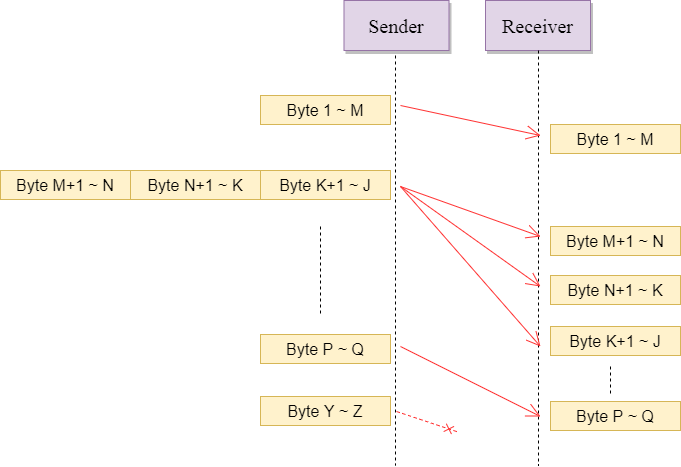
\includegraphics[scale=0.48]{Figures/namedpipe}}
\caption{Data Transfer Scenarios for Named Pipe}
\label{namedpipe}
\end{figure}

\subsubsection{Message Queue}
Message Queuing (MSMQ) is a communication method to allow applications which are running at different times across heterogeneous networks and systems that may be temporarily offline can still communicate with each other. Messages are sent to and read from queues by applications. Multiple sending applications can send messages to and multiple receiving applications can read messages from one queue.\cite{redkar2004pro} The applications are the endpoints of the communication. In this work, only one sending application versus one receiving application case is considered. Multiple senders to multiple receivers scenario can always be divided into multiple sender and receiver situation. Both endpoints of a communication can send to and receive from the channel.

The basic data transfer characteristics of Message Queue are:
\begin{itemize}
  \item Bytes sent in packet and received in packet, no bytes re-segmented
  \item Packets can lost
  \item Packets received in order
  \item No data duplication
\end{itemize}
Based on these characteristics,  the data transfer scenarios of Message Queue can be summarized in Figure\ref{msmq}.
\begin{figure}[H]
\centerline{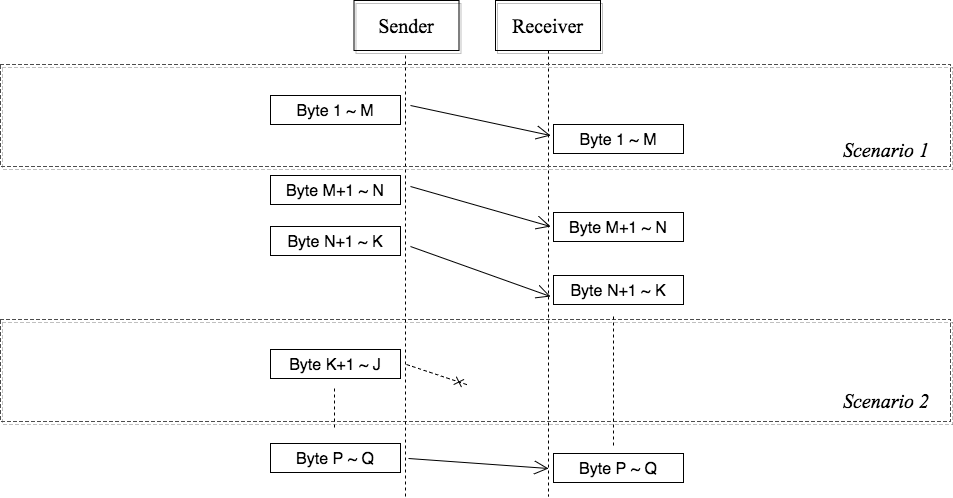
\includegraphics[scale=0.48]{Figures/msmq}}
\caption{Data Transfer Scenarios for Message Queue}
\label{msmq}
\end{figure}

\subsubsection{TCP}
TCP is the most fundamental reliable transport method in computer networking. TCP provides reliable, ordered, and error-checked delivery of a stream of octets between applications running on hosts in an IP network. The TCP header contains the sequence number of the sending octets and the acknowledge sequence this endpoint is expecting from the other endpoint(if ACK is set). The retransmission mechanism is based on the ACK. 

The basic data transfer characteristics of TCP are:
\begin{itemize}
  \item Bytes received in order
  \item No data lost(lost data will be retransmitted)
  \item No data duplication
  \item Sender window size is different from receiver's window size, so packets can be re-segmented
\end{itemize}

Based on these characteristics,  the data transfer scenarios of TCP can be summarized in Figure\ref{tcp}.
\begin{figure}[H]
\centerline{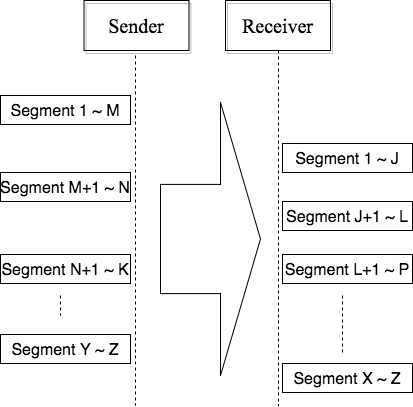
\includegraphics[scale=0.48]{Figures/tcp}}
 \caption{Data Transfer Scenarios for TCP}
\label{tcp}
\end{figure}

\subsubsection{UDP}
UDP is a widely used unreliable transmission method in computer networking. It is a simple protocol mechanism, which has no guarantee of delivery, ordering, or duplicate protection. This transmission method is suitable for many real time systems. 

The basic data transfer characteristics of UDP are:
\begin{itemize}
  \item Bytes sent in packet and received in packet, no re-segmentation
  \item Packets can lost
  \item Packets can be duplicated
  \item Packets can arrive receiver out of order
\end{itemize}

Based on these characteristics, the data transfer scenarios of UDP can be summarized in Figure\ref{upd}.
\begin{figure}[H]
\centerline{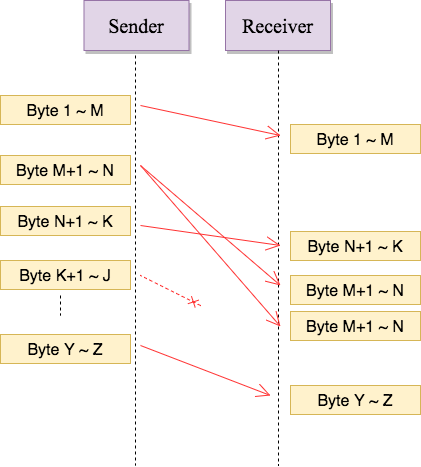
\includegraphics[scale=0.48]{Figures/udp}}
 \caption{Data Transfer Scenarios for UDP}
\label{upd}
\end{figure}

\section{Model of Communication}\label{definition}
This section define the communication of two programs. The communication in this work is data transfer activities between two running programs through a specific channel. Some collaborative activities between the programs such as remote procedure call is out of the scope of this research. Communication among multiple programs (more than two) is not discussed in this work. The channel can be reopened again to start new communications after being closed. However, the reopened channel will be treated as a new communication. The way that I define the communication is leading to the communication identification in the dual-trace. So the definition is not about how the communication works but what it looks like. There are many communication methods for the data transfer communications, but all of them are compatible to this communication definition. 

A communication $Co$ is defined by the 2-tuple $\langle ep, c \rangle$, where $ep$ is a set $\left\lbrace e_{x}: x= 0,1\right\rbrace $ for the two endpoints communicating with each other though the channel $c$. The endpoint $e_{x}$ is defined by the 3-tuple $\langle h_{x}, ds_{x}, dr_{x}\rangle$. $h_{x}$ is the handle created within a process for subsequent data transfer operations. $ds_{x}$ is the sequence of packets sent in the sending operations of $h_{x}$ while $dr_{x}$ is the sequence of packets received in the receiving operations of $h_{x}$. $e_{0}$ is created in process $p$ and $e_{1}$ is created in process $q$. Let $ds_{x} = \left(ps_{x,i}: 0\leqslant i \leqslant M_{x} \right)$ and $dr_{x} = \left(pr_{x,j}: 0\leqslant j \leqslant N_{x} \right)$ in which $ps_{x,i} = \langle ts_{x,i}, ss_{x,i} \rangle$ and $pr_{x,i} = \langle tr_{x,j}, sr_{x,j} \rangle$. $ts_{x,i}$ and $tr_{x,j}$ are the logical time when the packet being sent and received. $ss_{x,i}$ and $sr_{x,j}$ are the string payloads being sent and received. The string payloads can treated as sequence in the same order of the packets, $pls_{x} = \left(ss_{x,i}: 0\leqslant i \leqslant M_{x} \right)$ and $plr_{x} = \left(sr_{x,j}: 0\leqslant j \leqslant N_{x} \right)$. $\forall ps_{x,i} \in ds_{x}$, $ts_{x,k} \leqslant tr_{x,l}$ if $k \leqslant l$; $\forall pr_{x,i} \in dr_{x}$, $tr_{x,k} \leqslant tr_{x,l}$ if $k \leqslant l$; 

There are two sets of preservation of this definition. One set is for the reliable communication while the other is for the unreliable one. There are content preservation and timing preservation in each preservation set.

\textbf{Preservation for reliable communication:}
\begin{itemize}
 \item \textit{ Content Preservation:} Let $S_{x}$ be the concatenation of $\forall ss_{x,i} \in pls_{x}$ and $R_{x}$ be the concatenation of $\forall sr_{x,i} \in plr_{x}$. Then, $R_{0}$ is a sub string of $S_{1}$ and $R_{1}$ is a sub string of $S_{0}$.
 \item \textit{Timing Preservation:} Let $S_{x,k}$ be the concatenation of $\forall ss_{x,i} \in pls_{x}, 0 \leqslant k \leqslant M_{x}$ and $R_{x,l}$ be the concatenation of $\forall sr_{x,i} \in plr_{x}, 0 \leqslant l \leqslant N_{x}$. If $S_{0,k}$ is $R_{1,l}$, then $ts_{0,k} \leqslant tr_{1,l}$. If $S_{1,k}$ is $R_{0,l}$, then $ts_{1,k} \leqslant tr_{0,l}$. 
\end{itemize}

\textbf{Preservation for unreliable communication:}

$\forall sr_{0,j} \in plr_{0}, \exists ss_{1,i} \in pls_{1}$ and $\forall sr_{1,j} \in plr_{1}, \exists ss_{0,i} \in pls_{0}$ such that
\begin{itemize}
 \item \textit{ Content Preservation:}  $sr_{0,j} = ss_{1,i}$ and $sr_{1,j} = ss_{0,i}$ 
 \item \textit{Timing Preservation:}    $tr_{0,j} > ts_{1,i}$ and $tr_{1,j} > ts_{0,i}$
\end{itemize}
The terminology of using in this definition can be found in \ref{term}.



Figure\ref{communicationhappen} is a communication example of this definition. 
\begin{figure}[H]
\centerline{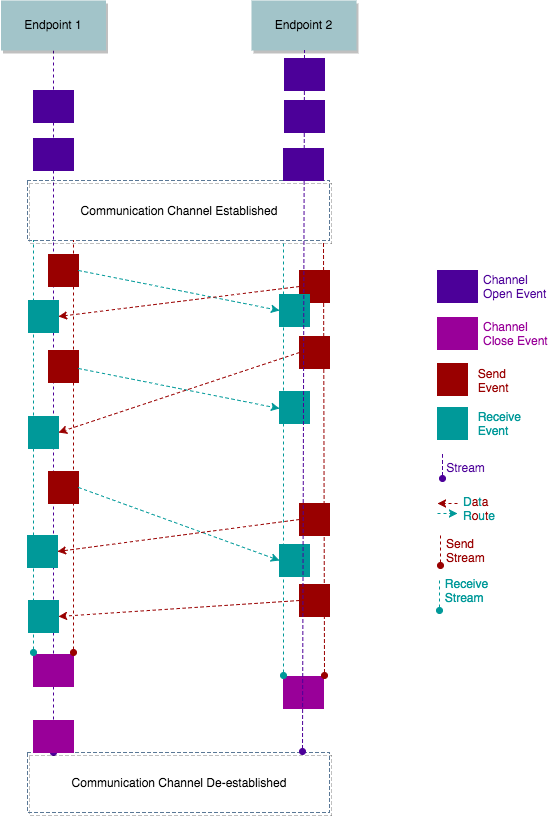
\includegraphics[scale=0.55]{Figures/communicationdefinition}}
\caption{Example of Communication}
\label{communicationhappen}
\end{figure}

\section{Model of the Dual-Trace of Two Communicating Programs}
The dual-trace being analysed are in assembly level. One dual-trace contains two execution traces. There is no timing information of these two traces which means we don't know the timestamps of the events of these two traces and can not match the events from both sides by time sequence. However the captured instructions in the trace are ordered in execution sequence. The execution traces contain all executed instructions as well as the corresponding changed memory by each instruction. Additionally, system calls are also captured by instruction id, which means if .dll or .exe files are provided, the system function calls can be identified with function names. Memory states can be reconstructed from the recorded memory changes to get the data information of the communication. In this section, I model the execution trace in the dual-trace. The communication identification is among the information of this model.

A dual-trace consist of two execution traces $\left\lbrace trace1, trace2 \right\rbrace $ . An execution trace is defined as a sequence $trace = (line_{k}, 0 \leqslant l \leqslant K)$. $line_{k}$ in a $trace$ is a 3\_tuple $\langle ins, mem, fi \rangle$ where $ins$ is the assembly instruction, $mem$ is memory changed by this instruction and $fi$ is function call information indicating if this is the function call or return. A function $eventfilter \left( \right) $ is defined to generate the event level trace $event_trace$ from the original $trace$. $event_trace = eventfilter\left( trace, funcset\right) $, where $funcset = \left \lbrace func_{l}, 0 \leqslant L \leqslant Q\right\rbrace $ is a set of the concerned events' function information.Each concerned event's function information can be described a tuple $langle funN, type, pars \rangle$ where $funN$ is the concerned event's function name, $type$ can only be one of these four event types: only be channel open, channel close, data send and data receive and $pars$, is the parameter information list. The output of this function $event_trace$ is a sequence of events $(event_{m}, 0 \leqslant l \leqslant M)$. Only the concerned events in the $funcset$ are filtered in this sequence, all other information in the original trace are ignored. Each event in the trace corresponds to a system function call and is defined as a 4\_tuple $\langle funN, startline, endline, type \rangle$. In this tuple $funN$ is the name of the called function, $startline$ is the line number where the function was being called, $endline$ is the line number where the function returned and $type$ is the event type. The events in the $event_trace$ are interleaving events among multiple handles. Function  $streamfilter \left( \right) $ is defined to generate the stream level trace $event_trace$ from the $event_trace$. $stream_trace =  eventfilter\left( event_trace \right) $. The output $stream_trace$ is a set of stream $\left \lbrace stream_{n}, 0 \leqslant n \leqslant N\right\rbrace$ in which each stream correspond to a handle and consist of 4 sub streams. So that $stream_{n} $ is a set  $\left \lbrace open_stream, send_stream, receive_stream, close_stream \right\rbrace $. Each of these sub streams consist of a sequence of $event$ of a certain handle of the corresponding event types.

\section{Element matching from Trace Modelling and Communication Modelling}
The goal of this work is to identify the communication from dual-trace. In the modelling, this can be abstracted as finding the elements of the communication model in the dual-trace model. The element matching can be summarized in Table\. By known this matching, algorithms can be developed to identify the communications in the dual-trace model. The developed algorithm will be discuss in next chapter.



